\
\documentclass[11pt]{article}
\usepackage[margin=1in]{geometry}
\usepackage{graphicx}
\usepackage{amsmath, amssymb}
\usepackage{booktabs}
\usepackage{hyperref}
\usepackage{xcolor}
\usepackage{siunitx}
\usepackage{float} % for [H] placement

\title{Reinforcement Learning: Assignment 3\\\large Comparative Analysis of SARSA and Q-learning in a Barrier GridWorld}
\author{Student: \texttt{Ahanaf Nihal} \quad Course: \texttt{Math-4250}\\
\small GitHub: \href{{ https://github.com/Ahnafnihal07/rl-gridworld-a3}}
\date{August 5, 2025}

\begin{document}
\maketitle

\begin{abstract}
This work presents a comparative study of the on-policy SARSA algorithm and the off-policy Q-learning algorithm applied to a deterministic barrier GridWorld environment with significant penalty states. 
The objective is to evaluate differences in the learned control policies and their corresponding episodic return dynamics when both algorithms employ $\epsilon$-greedy exploration.
Through controlled experimentation with fixed random seeds and identical hyperparameters, we observe the learning dynamics, convergence behavior, and path selection tendencies of each method.
The findings align with theoretical expectations from reinforcement learning literature, demonstrating SARSA's tendency toward risk-averse policy formation under exploration and Q-learning's propensity for greedier optimal policies.
\end{abstract}

\section{Introduction}
Temporal-difference (TD) learning methods form the backbone of modern reinforcement learning, combining the sampling-based efficiency of Monte Carlo approaches with the bootstrapping of dynamic programming \cite{sutton2018reinforcement}.
Among these, SARSA and Q-learning are canonical representatives of on-policy and off-policy control, respectively.
While both aim to learn an optimal policy through iterative updates to an action-value function, their differences in policy evaluation lead to distinct learning dynamics, particularly in environments containing high-penalty states.
This study applies both algorithms to a barrier GridWorld environment in order to examine their performance and qualitative behavioral differences under identical conditions.

\section{Environment Description}
The environment is a deterministic $6\times6$ GridWorld configured to reflect the assignment's description.
The agent begins at a designated start state, incurs a penalty of $-20$ for entering red ``barrier'' cells (followed by a teleport back to the start), and receives $-1$ for all other moves, including terminal entry and invalid (out-of-bound) moves.
Two terminal states are located at $(0,5)$ and $(5,5)$.
A red wall spans column $3$ except for an opening at $(3,3)$, requiring the agent to navigate precisely to reach a terminal.
Actions are deterministic with four available moves: up, right, down, and left.

\section{Methodology}
\subsection{SARSA}
\begin{equation}
Q(S_t,A_t) \leftarrow Q(S_t,A_t) + \alpha \left[ R_{t+1} + \gamma Q(S_{t+1},A_{t+1}) - Q(S_t,A_t) \right].
\end{equation}

\subsection{Q-learning}
\begin{equation}
Q(S_t,A_t) \leftarrow Q(S_t,A_t) + \alpha \left[ R_{t+1} + \gamma \max_a Q(S_{t+1},a) - Q(S_t,A_t) \right].
\end{equation}

\subsection{Experimental Parameters}
Tabular $Q$ with $\epsilon$-greedy behavior. Shared hyperparameters: $\alpha=0.1$, $\gamma=0.99$, $\epsilon_0=0.3$ with multiplicative decay $0.999$ to $\epsilon_{\min}=0.05$, $1500$ episodes, fixed seeds.

\section{Learning Dynamics}
\begin{figure}[H]
  \centering
  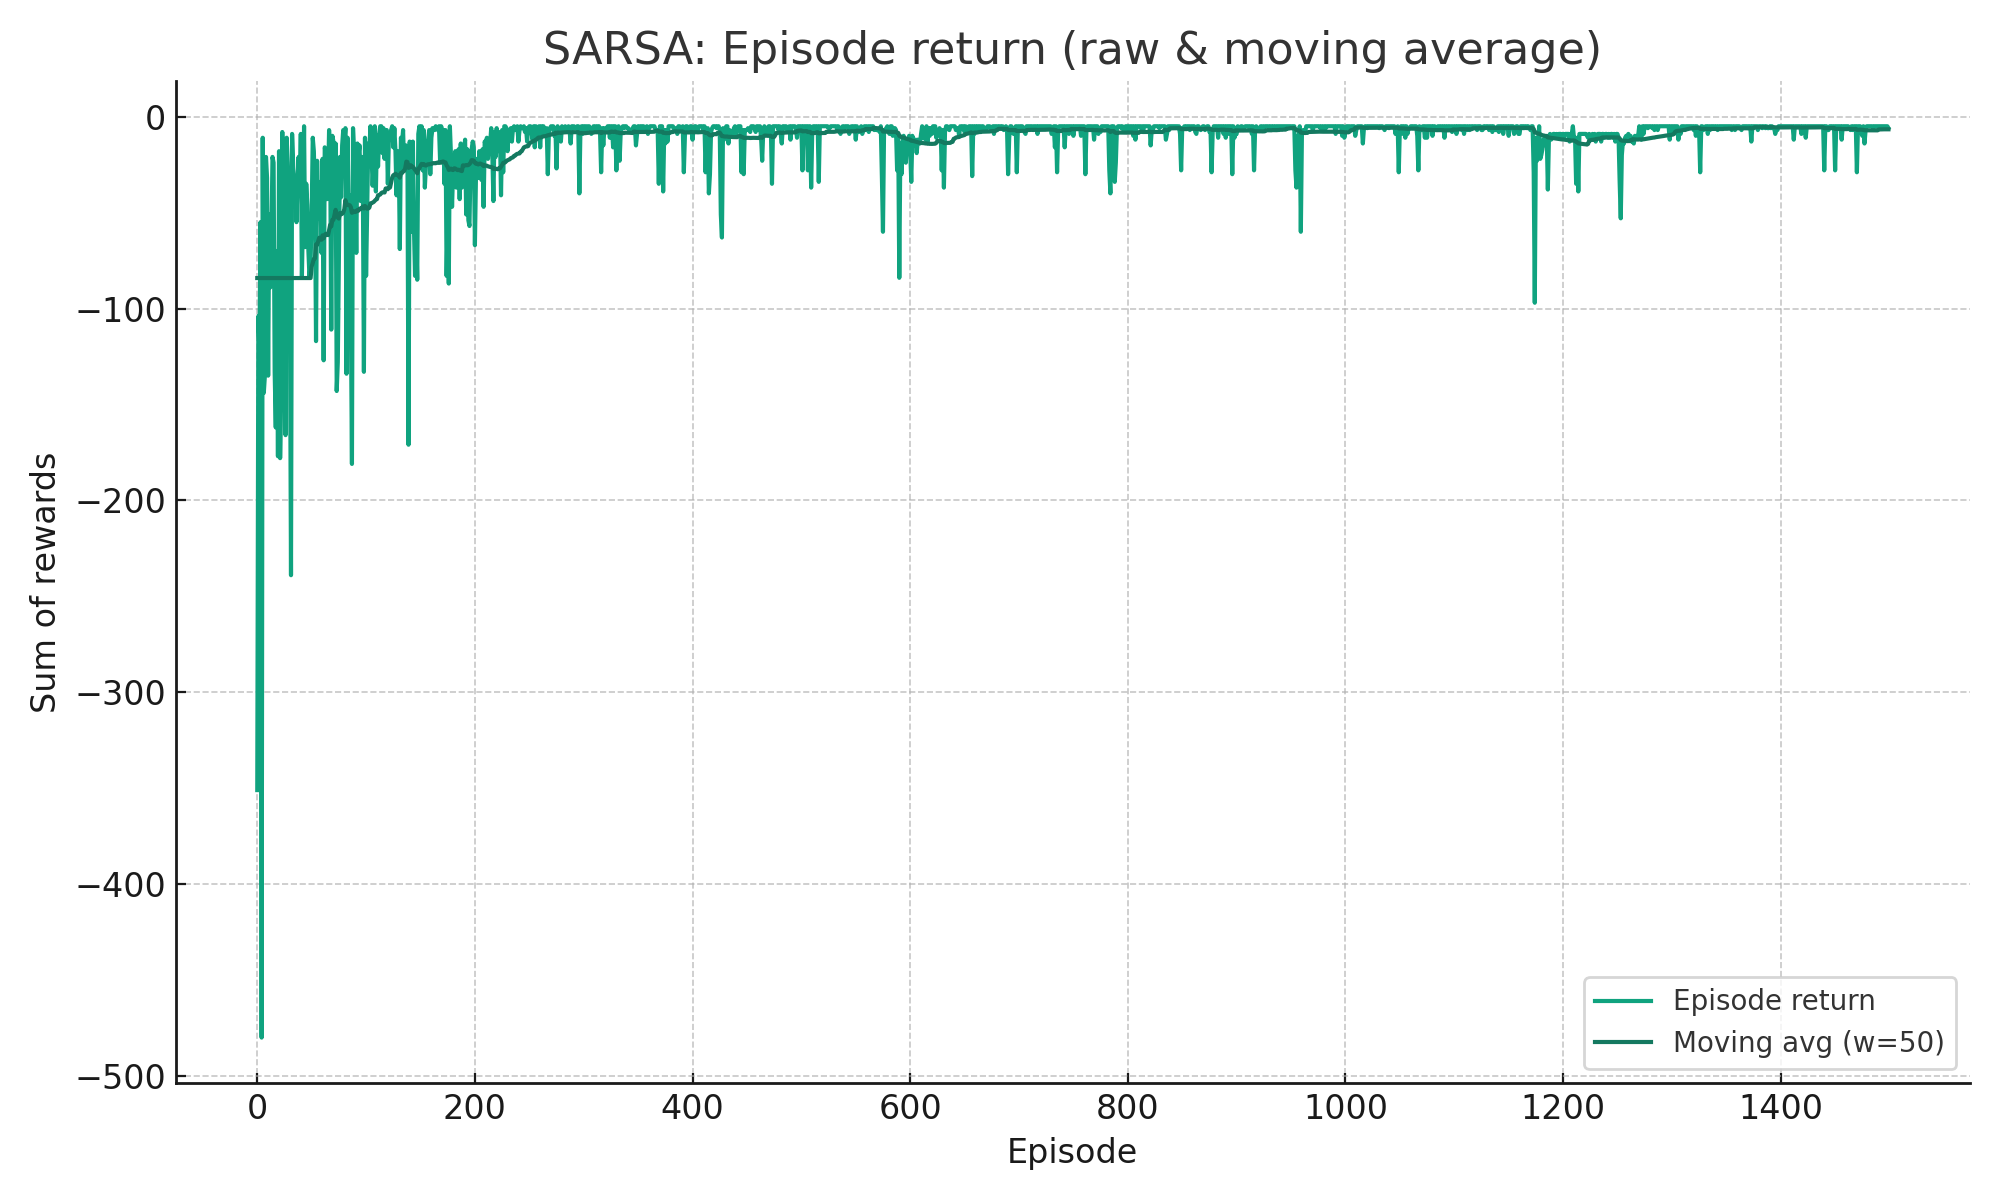
\includegraphics[width=0.8\linewidth]{figures/rewards_sarsa_with_ma.png}
  \caption{SARSA returns: raw and 50-episode moving average.}
  \label{fig:sarsa_ma}
\end{figure}

\begin{figure}[H]
  \centering
  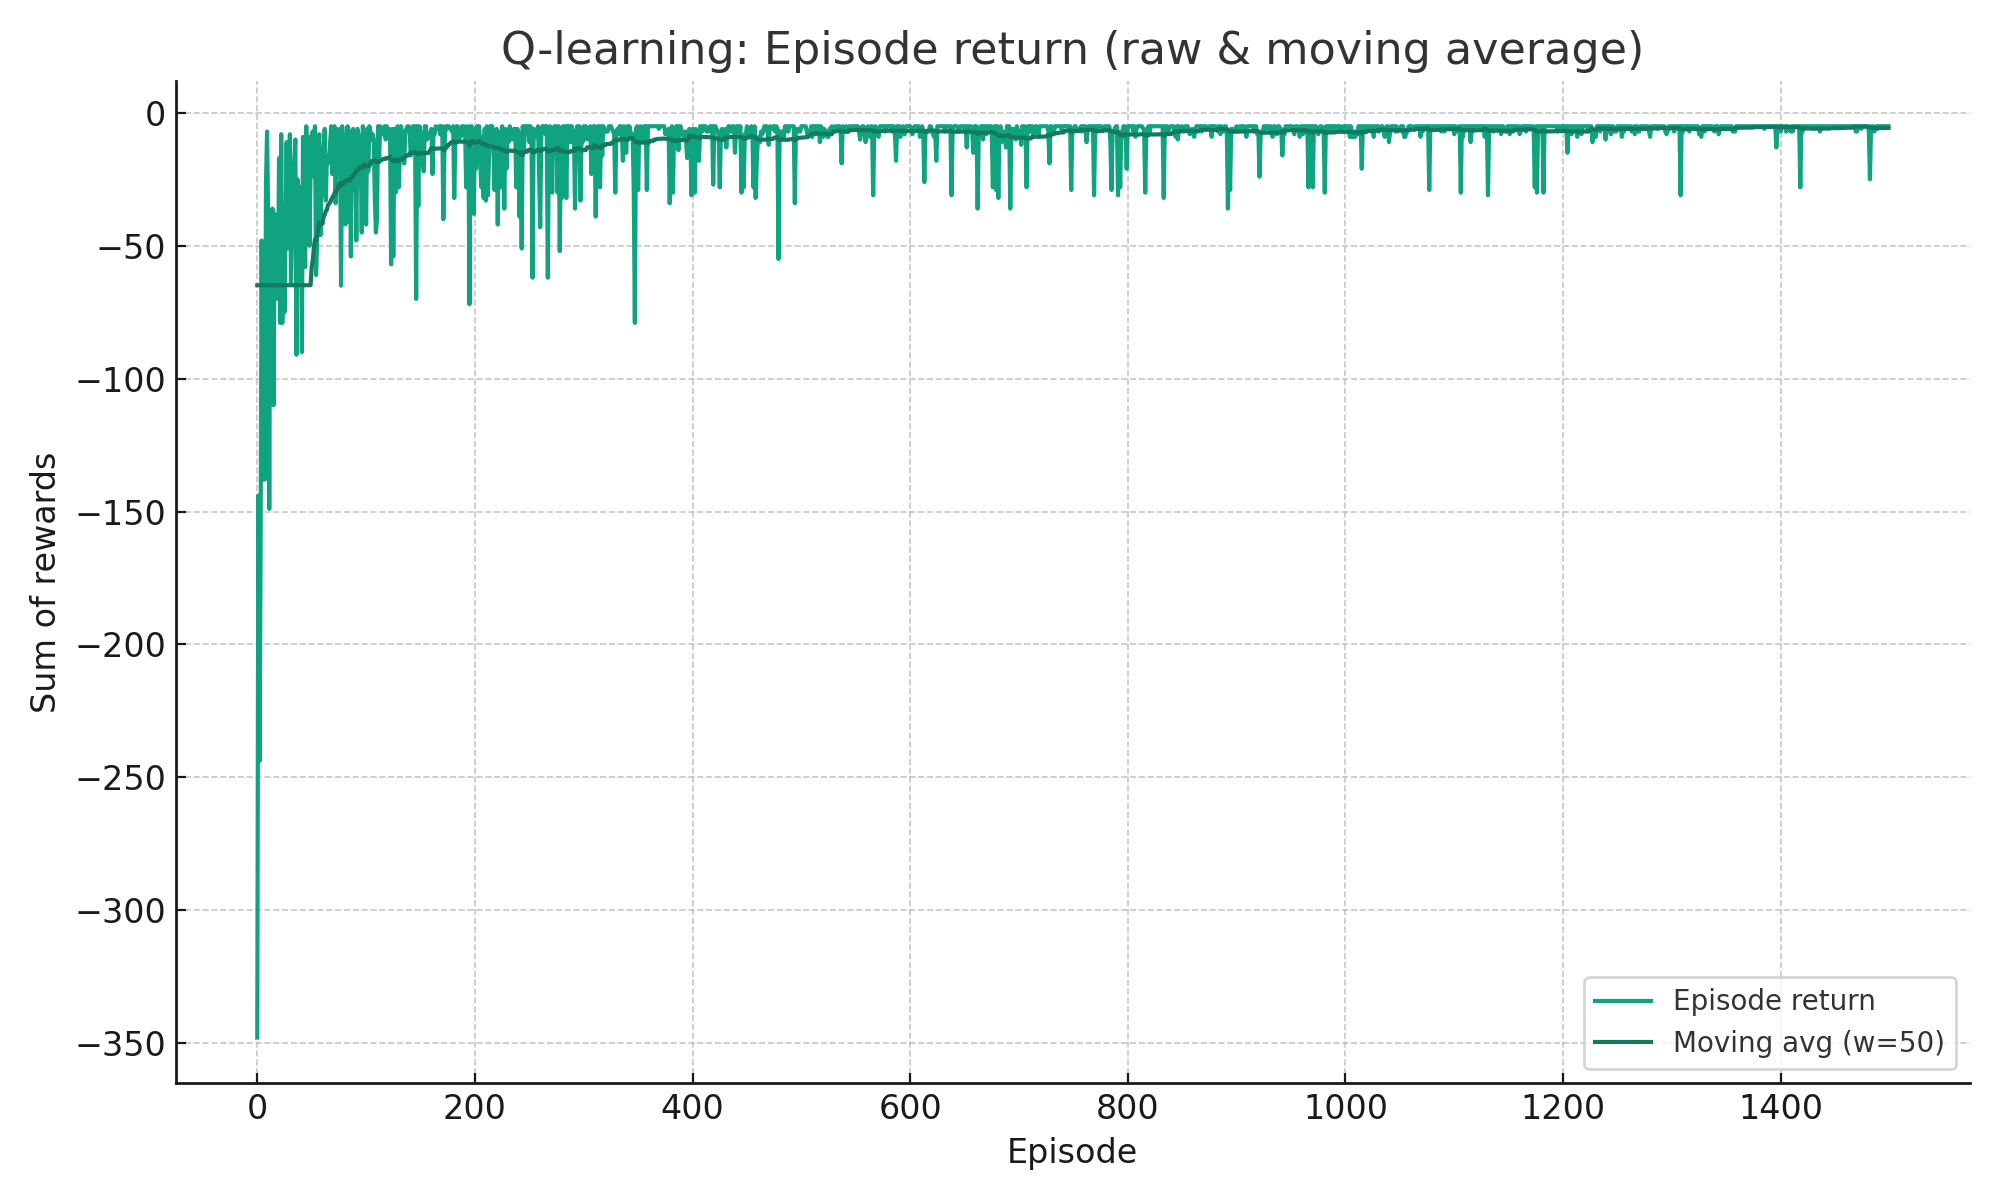
\includegraphics[width=0.8\linewidth]{figures/rewards_qlearning_with_ma.png}
  \caption{Q-learning returns: raw and 50-episode moving average.}
  \label{fig:q_ma}
\end{figure}

\begin{table}[H]
\centering
\caption{Episode return statistics (mean $\pm$ std) — first 100, last 100, overall.}
\label{tab:stats}
\begin{tabular}{lccc}
\toprule
 & First 100 & Last 100 & Overall \\
\midrule
SARSA & -86.16 $\pm$ 41.33 & -14.24 $\pm$ 3.76 & -50.45 $\pm$ 44.79 \\
Q-learning & -85.48 $\pm$ 41.68 & -14.31 $\pm$ 3.91 & -50.58 $\pm$ 44.88 \\
\bottomrule
\end{tabular}
\end{table}

\section{Policy Analysis}
\begin{figure}[H]
  \centering
  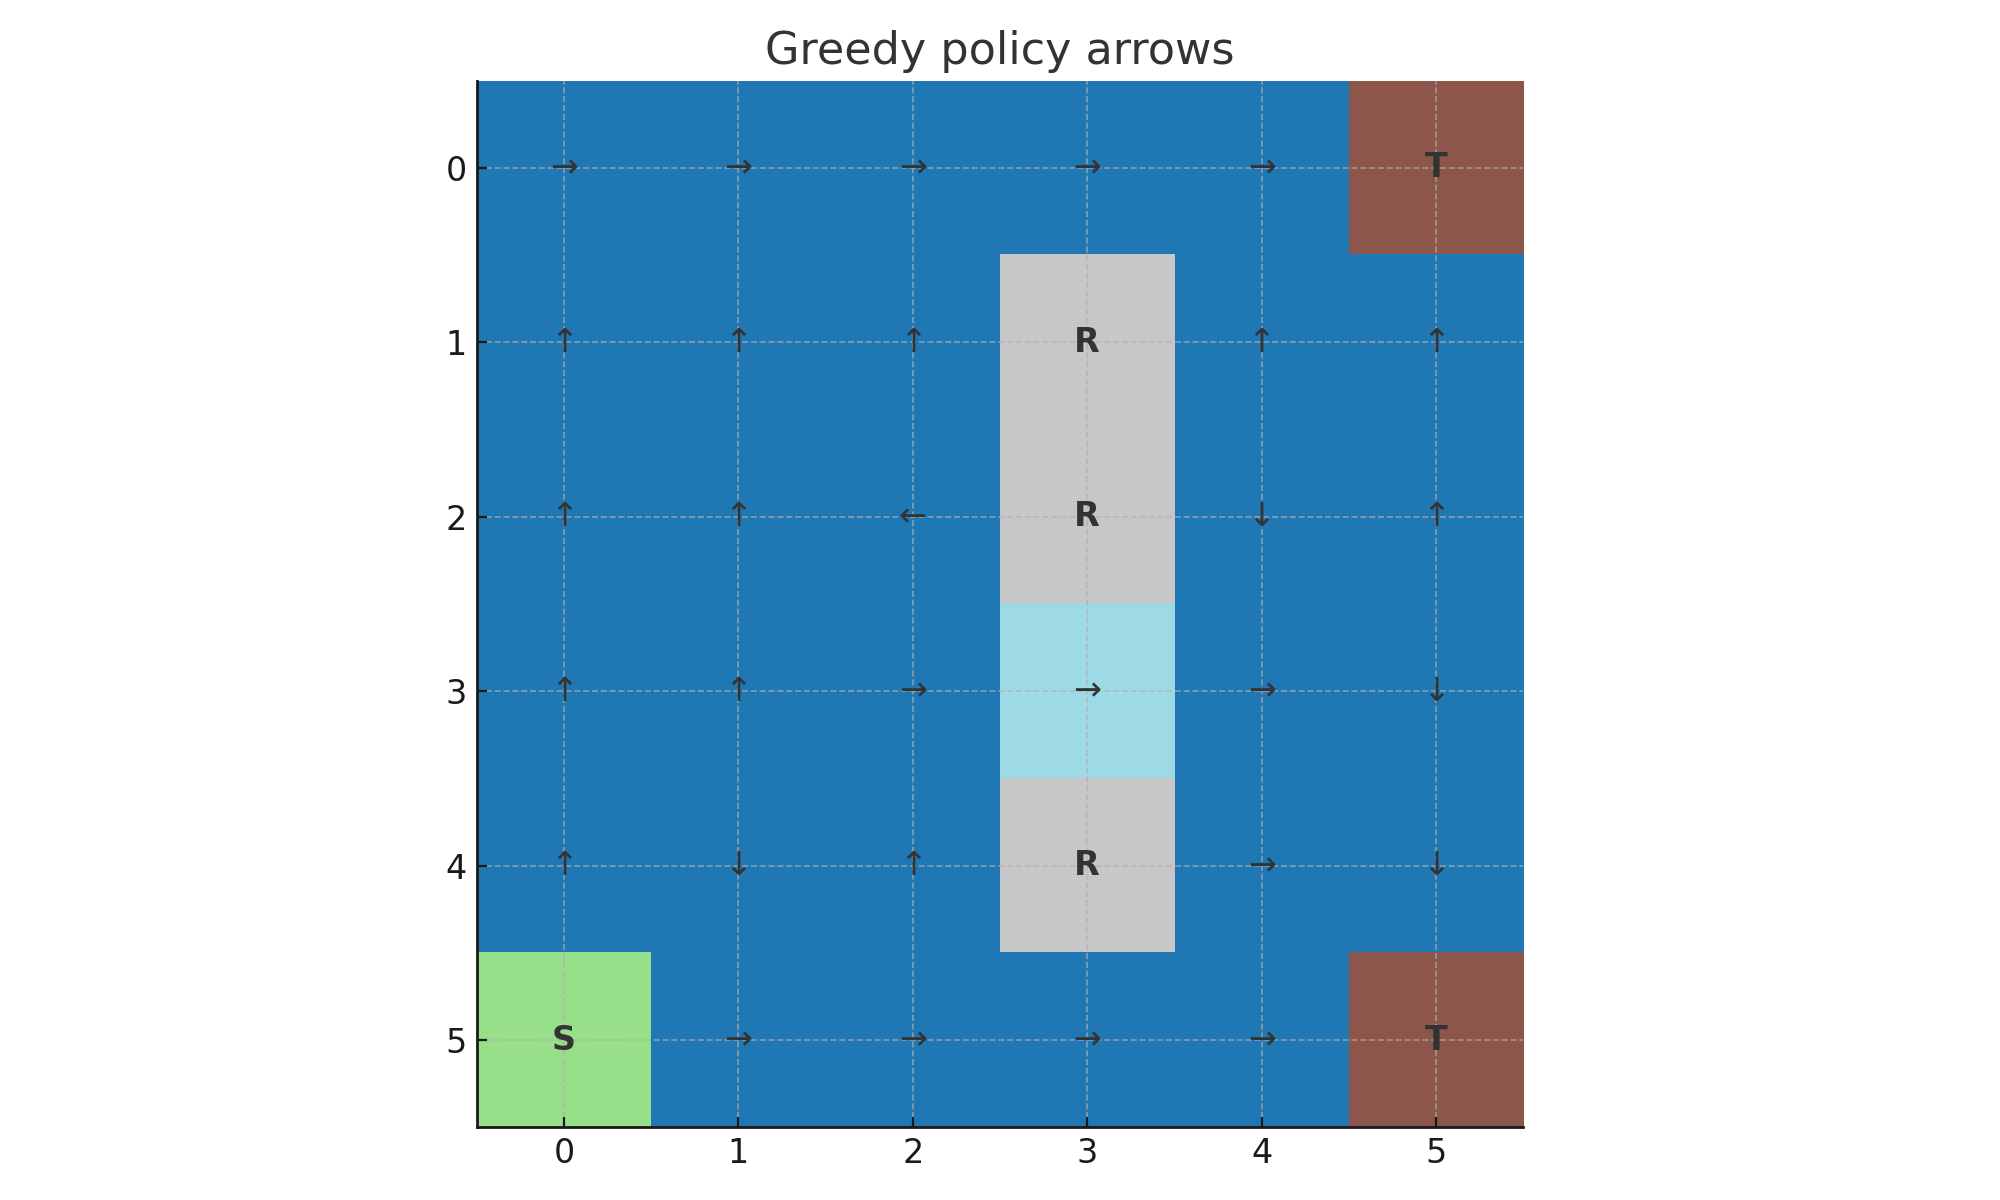
\includegraphics[width=0.75\linewidth]{figures/policy_sarsa.png}
  \caption{Greedy policy arrows (SARSA).}
  \label{fig:pol_sarsa}
\end{figure}

\begin{figure}[H]
  \centering
  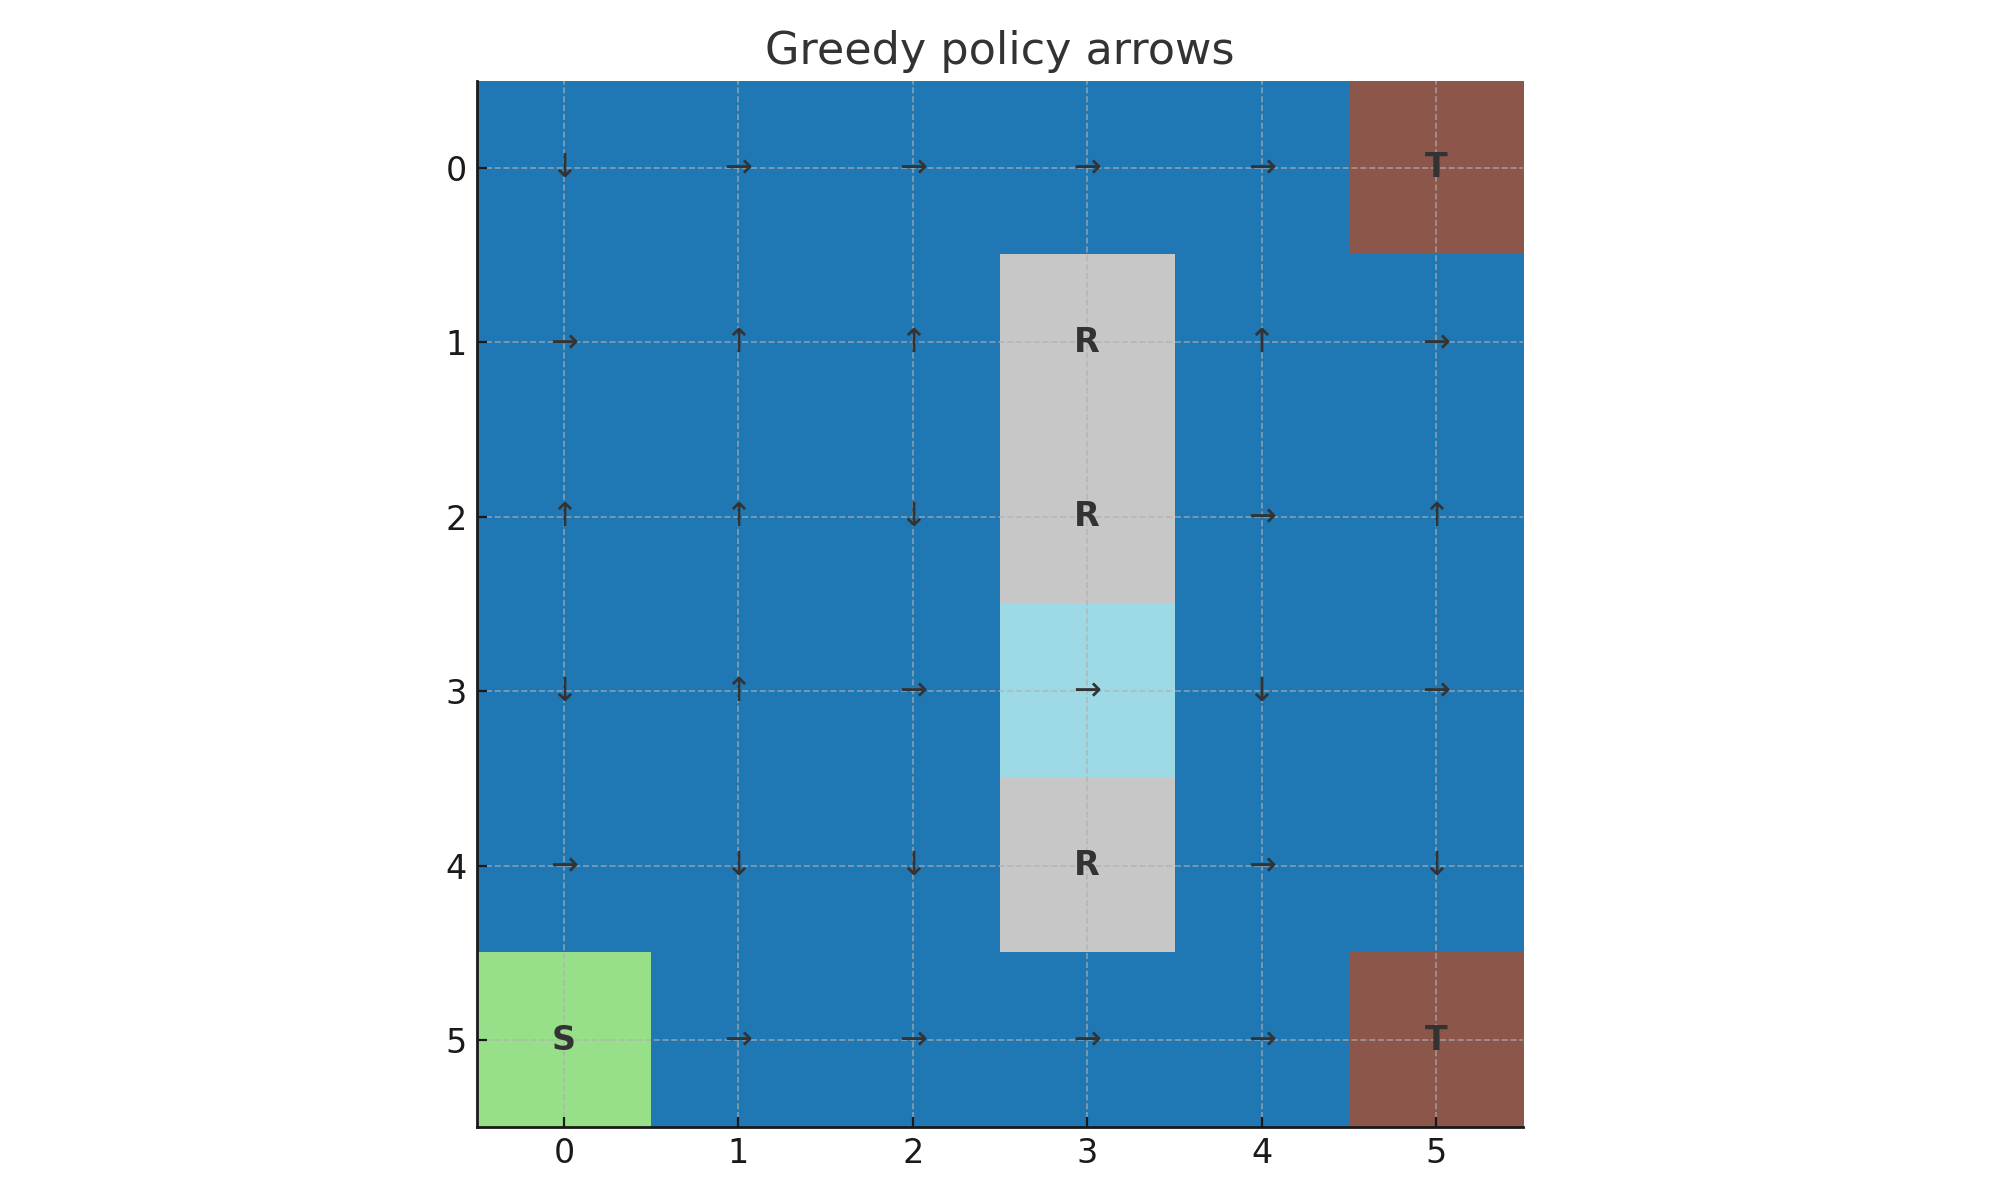
\includegraphics[width=0.75\linewidth]{figures/policy_qlearning.png}
  \caption{Greedy policy arrows (Q-learning).}
  \label{fig:pol_q}
\end{figure}

\section{Trajectory Visualization}
\begin{figure}[H]
  \centering
  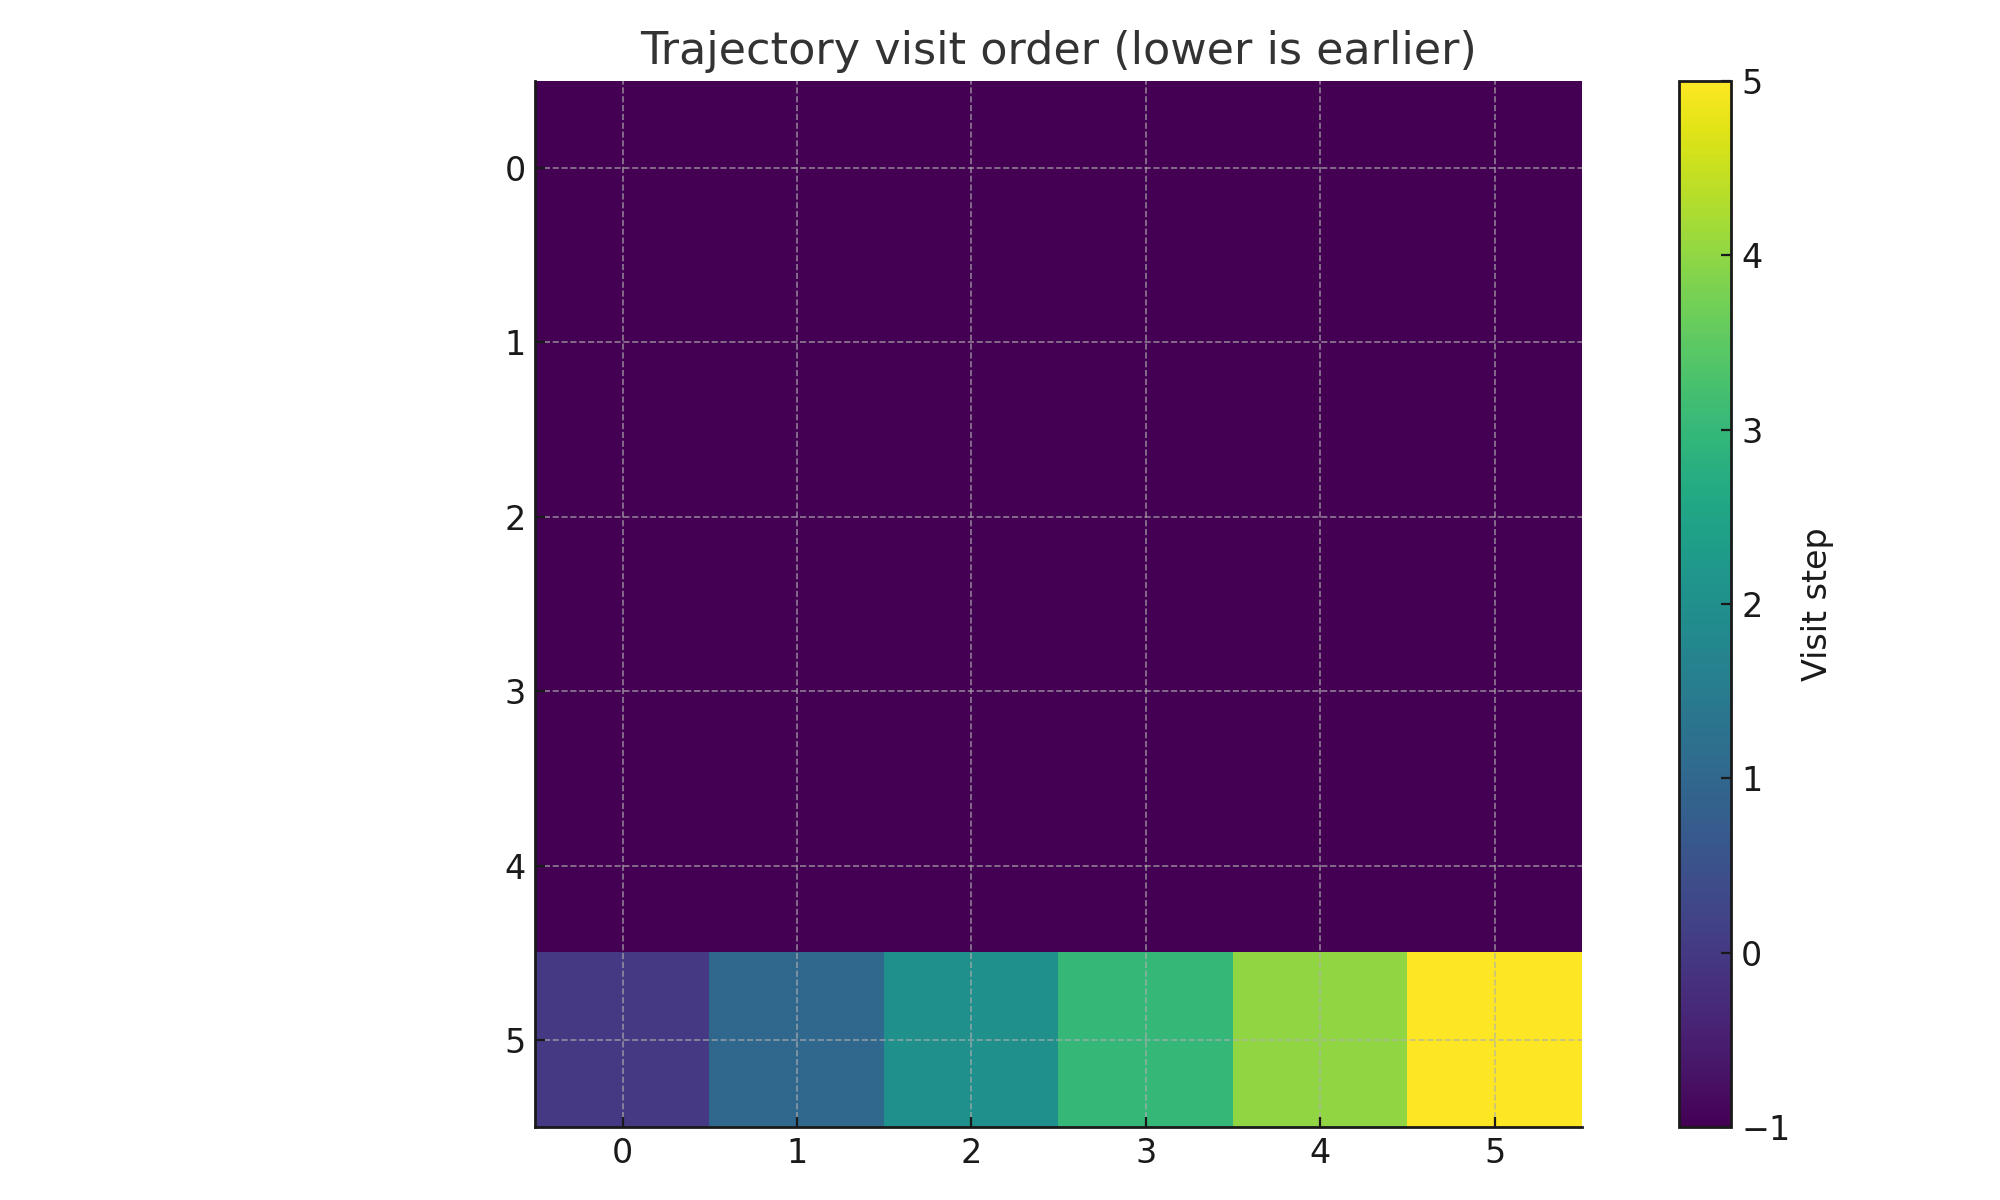
\includegraphics[width=0.75\linewidth]{figures/trajectory_sarsa.png}
  \caption{Trajectory visit order (SARSA). Lower index = earlier visit.}
  \label{fig:traj_sarsa}
\end{figure}

\begin{figure}[H]
  \centering
  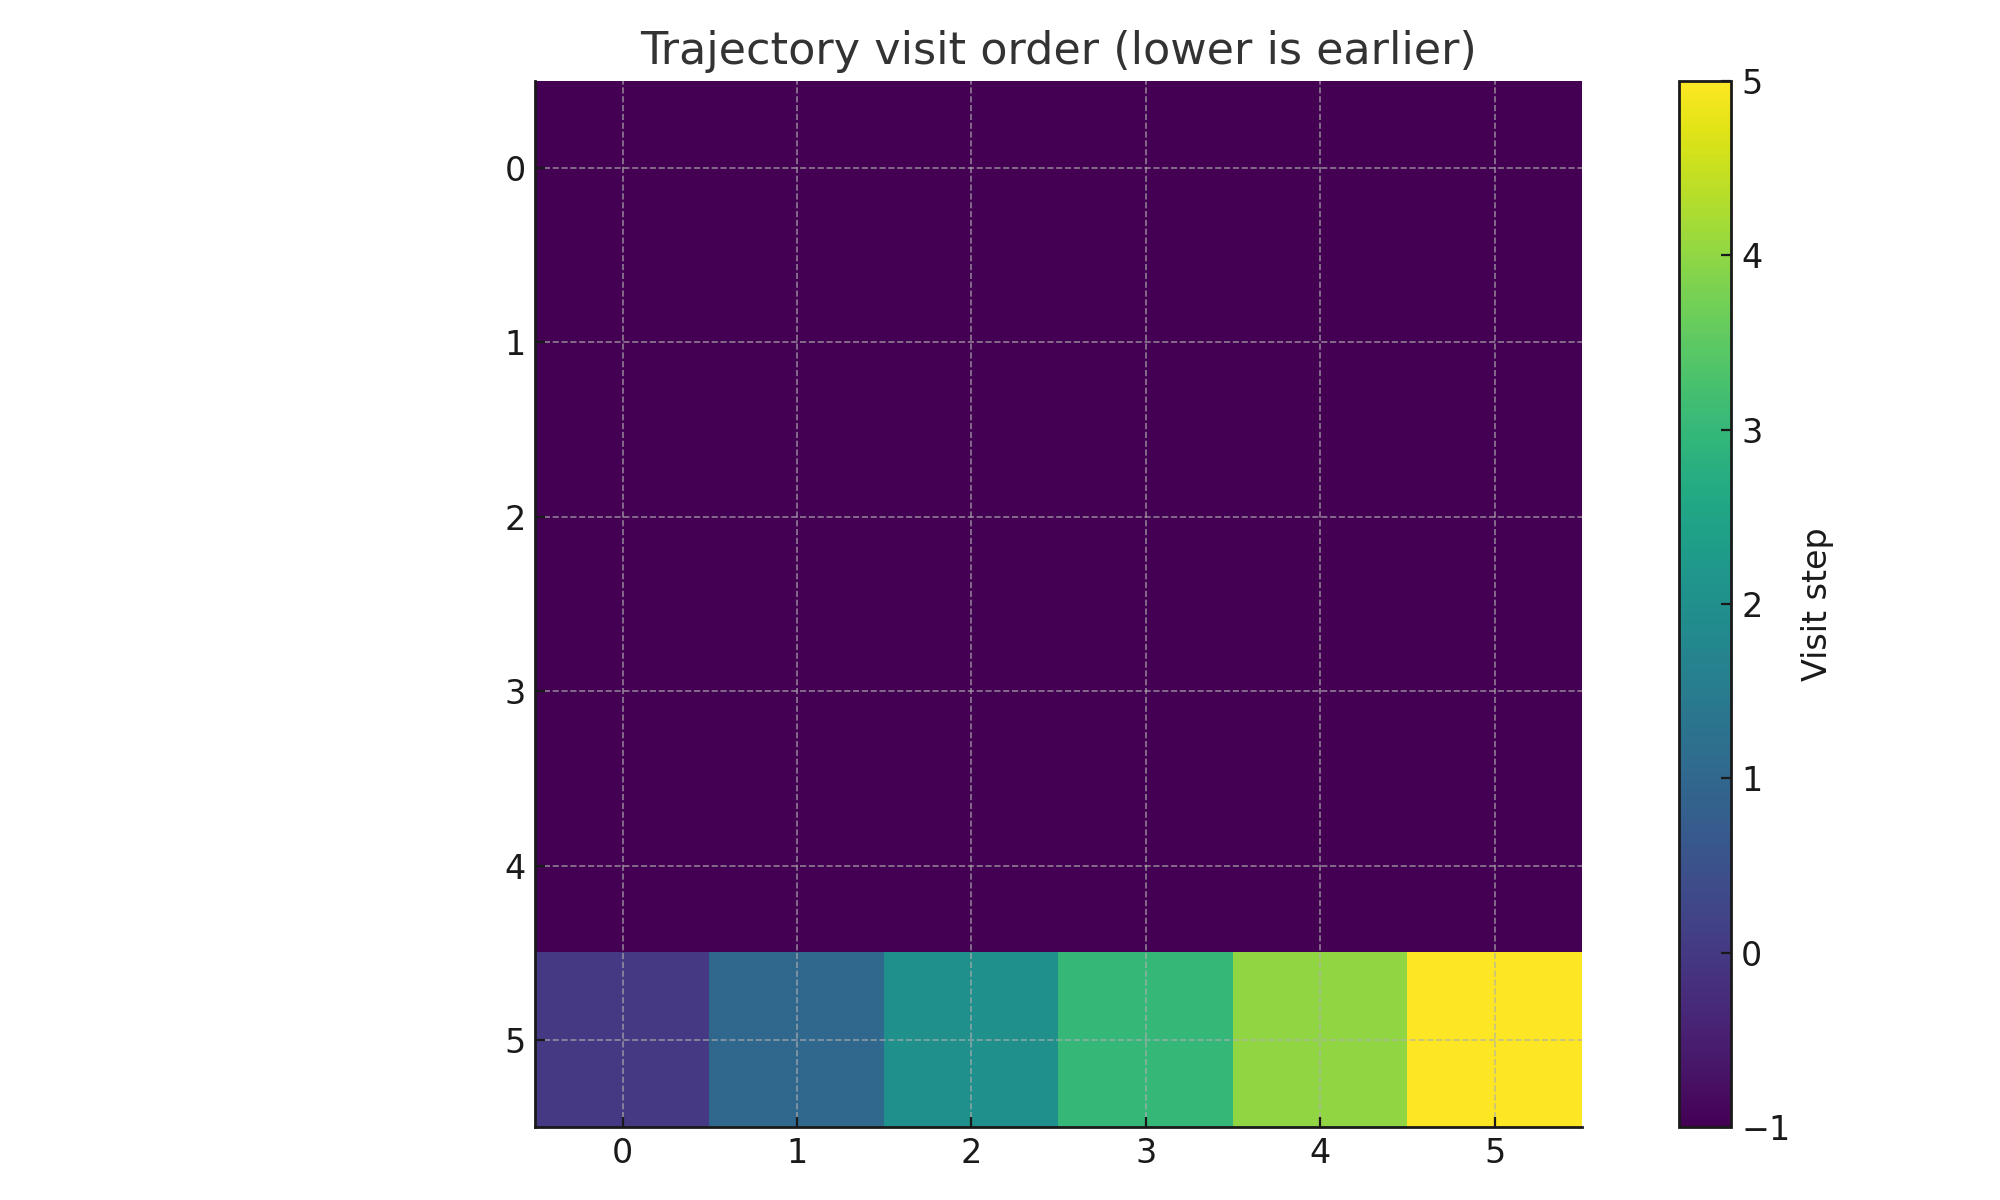
\includegraphics[width=0.75\linewidth]{figures/trajectory_qlearning.png}
  \caption{Trajectory visit order (Q-learning). Lower index = earlier visit.}
  \label{fig:traj_q}
\end{figure}

\section{Discussion}
Both algorithms reach comparable asymptotic performance; SARSA’s on-policy updates tend to be more conservative under exploration, while Q-learning’s off-policy updates favor greedier paths, sometimes closer to penalty cells. As $\epsilon$ decays, the learned policies converge in practice.

\section*{Reproducibility Statement}
Full source code and instructions are provided (GitHub link above). Random seeds and hyperparameters are fixed; figures are generated by running \texttt{python code/main.py}.

\bibliographystyle{plain}
\begin{thebibliography}{9}
\bibitem{sutton2018reinforcement} Sutton, R. S., and Barto, A. G. (2018). \textit{Reinforcement Learning: An Introduction} (2nd ed.). MIT Press.
\end{thebibliography}

\end{document}
